\FrontmatterChapter{Resumen}
{\setlength{\parindent}{0pt}
\begin{Large}
\textbf{OPTIMIZACIÓN DEL SISTEMA DE VISIÓN ARTIFICIAL DE UN ROBOT INDUSTRIAL PARA UNA APLICACIÓN DE PICK AND PLACE}
\end{Large}

\textbf{Autor: Ortiz de Zúñiga Mingot, Ignacio.} \\
Directores: Boal Martín-Larrauri, Jaime y Rodríguez Mondéjar, José Antonio. \\
Entidad colaboradora: ICAI – Universidad Pontificia Comillas \\

\section*{Resumen del proyecto}
En la última década se ha producido revolución industrial conocida como industria 4.0 gracias a los numerosos avances en el sector de la robótica. Este cambio se ha visto producido gracias a que con el desarrollo de los robots se ha conseguido dotar a estos de capacidades para completar tareas previamente imposibles para el ser humano y con un rendimiento y rapidez superior. Es por ello que se decidió implantar dichos sistemas en un robot industrial de Comillas ICAI con el fin de que este sea capaz de recolectar piezas de LEGO dispuestas de forma aleatoria sobre una mesa de trabajo. En este proyecto se parte de este sistema basado en la segmentación clásica y se mejora y actualiza con el desarrollo de sistemas basados en redes neuronales y aprendizaje profundo. Se han desarrollado múltiples redes de diferentes tamaños basadas en R-CNN, Faster R-CNN y YOLO y se camparan entre si y frente al sistema de segmentación clásico. \\
\textbf{Palabras clave:} Visión artificial, Redes neuronales, AlexNet, VGG-16, R-CNN, Faster R-CNN, YOLO, Robótica, LEGO

\section*{1. Introducción}
Durante los últimos dos años se ha desarrollado un sistema que dote de visión artificial y autonomía a los robots de Comillas ICAI. La tarea escogida para llevar a cabo con estos robots es la recolección de piezas de LEGO dispuesta de forma aleatoria en una zona de trabajo. Este proyecto surge como la evolución de estos sistemas con el fin de mejorar el subsistema de visión artificial mejorando así las capacidades del robot. Para ello primero se ha mejorado el sistema presente con el desarrollo de nuevos análisis más detallados y precisos. Este sistema se basa en el filtrado con máscaras de color, la detección de bordes y la transformada de Hough. Además, se han desarrollado nuevos sistemas para el cálculo de la profundidad y el cálculo de la orientación de la pieza. Sin embargo, a pesar de estas mejoras se ha observado que este sistema no puede competir con los sistemas más modernos ya implantados en la industria. Es por ello que se han desarrollado nuevos sistemas basados en redes neuronales convolucionales. Tal y como su nombre indica estos se basan en el principio de la convolución y el aprendizaje profundo. Con la ayuda de una base de datos son capaces de extraer las características de un objeto y aprender a identificarlo. Es por ello que se a optado por dotar de esta tecnología a los sistemas previos para mejorarlos y así perfeccionar los.

\section*{2. Metodología}
El sistema de visión artificial implantado en el brazo robótico esta constituido por tres elementos que deben de cooperar entre si y comunicarse a través de conexiones USB y TCP/IP. La captura de imágenes se realiza con una cámara Intel Realsense D435 que cuenta con sensores RGB y de profundidad y ha sido conectada a través de una conexión USB. El procesado de las imágenes RGB y de profundidad es llevado a cabo por un ordenador con la ayuda de MATLAB. Y por último,se mandarán las instrucciones conteniendo la posición, altura y orientación de cada pieza a través de una conexión TCP/IP al brazo robótico IRB 120. Esta estructura se puede ver en la \autoref{fig:resm1}

\begin{figure}[ht]
	\centering
	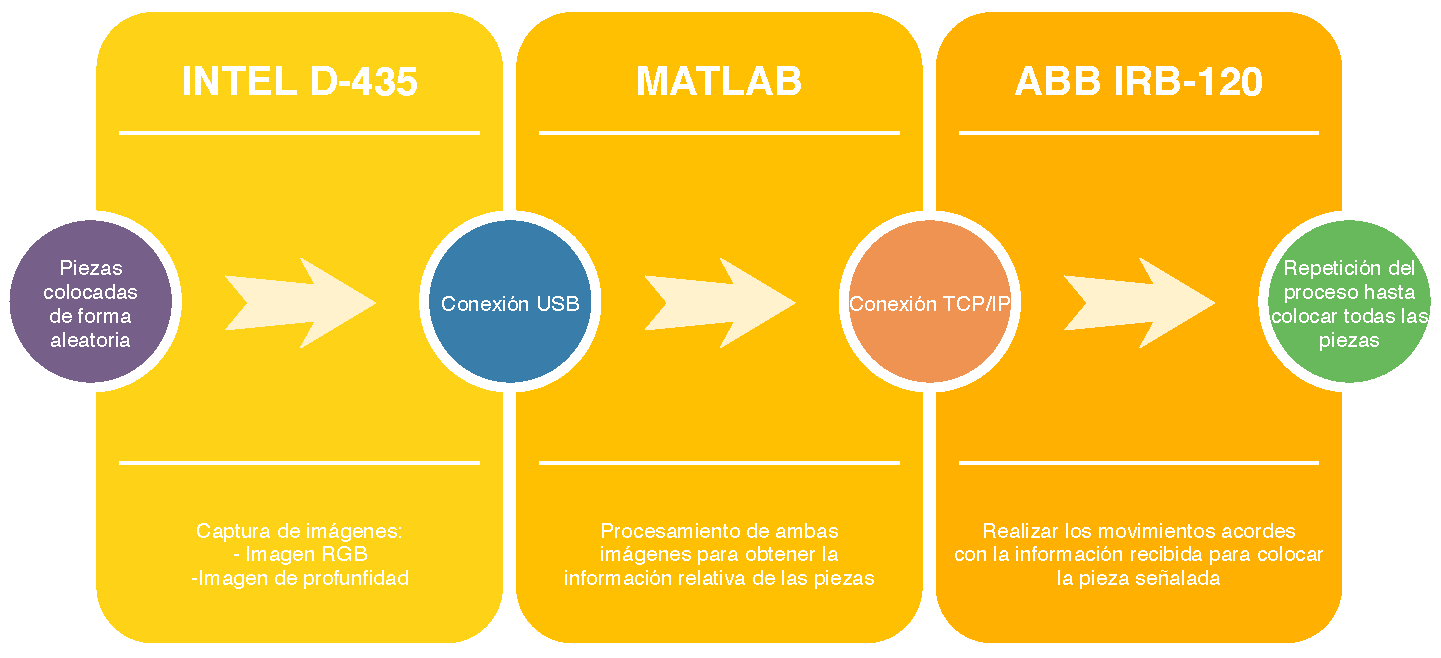
\includegraphics[width=0.9\textwidth]{Introduccion/Esquema_arquitectura.pdf}
	\caption{Esquema de la arquitectura del sistema}
	\label{fig:resm1}
	\vspace{-5pt}
\end{figure}

El primer paso en el desarrollo de este proyecto ha sido la mejora el sistema actual basado en filtros con máscaras de color, la detección de bordes y la transformada de Hough. Se han revisado los filtros de color reduciendo así los falsos positivos y se ha perfeccionado el análisis por detección de bordes de las piezas. Se ha rediseñado y calibrado la cámara para permitir una captura más rápida y eliminar las distorsiones presentes en la imagen de profundidad. También se ha rediseñado el sistema de cálculo de la orientación con el desarrollo de un análisis más exhaustivo de todas las caras de las piezas de LEGO mediante la transformada de Hough.

Una vez este sistema ha sido mejorado y perfeccionado, se ha desarrollado desde cero nuevos detectores de objetos basados en redes neuronales convolucionales. Con el fin de poder realizar un análisis riguroso de estas redes y poder seleccionar un buen método o combinación de métodos a emplear, se han desarrollado múltiples redes de diferentes tamaños y basadas en diferentes tecnologías. Las redes desarrolladas son del tipo: tipo R-CNN, Faster R-CNN y YOLO. Y para cada tipo de tecnología se han creado dos redes basadas en clasificadores reentrenados basados en AlexNet y VGG-16.

Para poder llevar esto a cabo es necesario primero rediseñar y reentrenar los clasificadores antes de poder crear los detectores de objetos. El motivo por el que se ha llevado a cabo este paso es que es común y altamente recomendable a la hora de desarrollar un detector de objetos, que este sea basado en un clasificador. Este proceso es conocido como aprendizaje por transferencia y ayuda a reducir el tiempo de entrenamiento y el número de datos necesarios a la vez que mejora los resultados. Es por ello que en este proyecto se ha decidido emplear el aprendizaje por transferencia partiendo de dos clasificadores diferentes. Los clasificadores empleados son AlexNet y VGG-16, sin embargo, estos clasificadores no han sido entrenados para la identificación de piezas de LEGO. Es por ello que primero serán reentrenados para la identificación de dichas piezas. Y a continuación, se partirá de estos dos nuevos clasificadores bautizados como LEGONet y LEGO16 para el desarrollo de los detectores de objetos mencionados previamente. Es decir, dos redes del tipo R-CNN, dos del tipo Faster R-CNN y dos del tipo YOLO.

R-CNN surgió como evolución de los primeros detectores de objetos basados en ventanas flotantes. Esta red primero analiza la imagen y determina aproximadamente 2000 regiones de interés para que estas sean analizadas de forma independiente por un clasificador. Con este sistema se redujo los tiempos de ejecución frente a los previos sistemas, pero sigue siendo un sistema lento ya que debe de analizar cada sección por separado. A cambio de un mal rendimiento, se caracteriza por ser uno de los sistemas más precisos y capaces. Durante el desarrollo de este proyecto se han desarrollado dos redes tipo R-CNN basadas en LEGONet y LEGO16. Estas redes han sido entrenadas con una base de datos desarrollada por nosotros y se han realizado múltiples pruebas con el fin de determinar las mejores opciones de entrenamiento.

Faster R-CNN surge tres años después de R-CNN como una evolución del mismo. Al igual que R-CNN se basa en la propuesta de regiones pero este proceso es llevado a cabo por una red RPN, una red neuronal convolucional cuya salida son las regiones de interés. Esta red se basa en la información extraída por las primeras capas del clasificador. El análisis de las regiones de interés también se lleva a cabo con el resto del clasificador y de forma independiente. En este sistema no se tiene que analizar la imagen original tantas veces como regiones propuestas sino que solo se analizan las regiones de interés extraídas de las capas de convolución iniciales. Y es por ello que se consigue reducir los tiempos de ejecución. Durante el desarrollo de este proyecto se han desarrollado dos redes tipo Faster R-CNN basadas en LEGONet y LEGO16. Estas redes han sido entrenadas con una base de datos desarrollada por nosotros y se han realizado múltiples pruebas con el fin de determinar las mejores opciones de entrenamiento.

YOLO es uno de los sistemas más modernos y actuales empleados para la detección de objetos. Se caracteriza por su rapidez de entrenamiento y de ejecución. Esto se debe a que tal y como su nombre indica, \textit{You Only Look Once}, es un tipo de red en la que la imagen solo se analiza una vez. Y mediante el uso de de un sistema de predicción de \textit{bounding boxes} determina los objetos presentes en la imagen. Este sistema se caracteriza porque a diferencia de los sistemas mencionados anteriormente, es capaz de ver toda la imagen a la vez y por ello puede establecer relaciones entre \textit{bounding boxes}.. Durante el desarrollo de este proyecto se han desarrollado dos redes tipo YOLO basadas en LEGONet y LEGO16. Estas redes han sido entrenadas con una base de datos desarrollada por nosotros y se han realizado múltiples pruebas con el fin de determinar las mejores opciones de entrenamiento.

Una vez identificadas todas las piezas mediante el uso de los detectores de objetos, es necesario calcular su orientación y altura. Este proceso ya ha sido perfeccionado al principio del proyecto. La información obtenida con todos estos análisis es mandada al brazo robótico y las piezas detectadas son recolectadas.

Como desarrollo adicional del proyecto, se ha decidido crear dos modelos de regresión basados en LEGONet y LEGO16 con el fin de estimar la orientación de una pieza de LEGO. Para el desarrollo de estas redes se ha preparado una nueva base de datos desarrollada por nosotros y constituida por miles de imágenes de piezas de LEGO rotadas diferentes ángulos. Para el entrenamiento también se han llevado a cabo múltiples pruebas con el objetivo de encontrar las mejores opciones de entrenamiento.

\section*{3. Resultados}
\subsection*{Detectores de objetos}
Tras desarrollar y entrenar todos los sistemas para la detección de objetos, se ha llevado a cabo una comparativa enfrentado los entre sí y frente a la versión mejorada del sistema clásico. Para la evaluación se han analizado un total de 380 piezas de LEGO de diferentes colores y en diferentes escenas. Con la evaluación se han llevado a cabo múltiples mediadas para evaluar el comportamiento de cada sistema.

\subsubsection*{Precisión, Exhaustividad, Tasa de fallos y FPPI}
Como se ha mencionado anteriormente, se han medido diferentes parámetros para evaluar el comportamiento de cada sistema. La precisión indica el nivel de similitud entre la detección de cada método y la verdadera región en la que se encuentra la pieza. La exhaustividad determina la relación entre los verdaderos positivos y los falsos negativos. La tasa de fallos determina la probabilidad de no detectar una de las piezas de LEGO. Y FPPI representa el número de falsos positivos por imagen detectadas. Tras evaluar todos los sistemas desarrollados, se puede observar la clara superioridad de las redes neuronales. Los nuevos sistemas son capaces de detectar piezas de LEGO bajo diferentes escenarios y condiciones lumínicas. Además, han reducido notablemente el número de falsos positivos y la tasa de fallo. Y entre ellos destaca R-CNN por su precisión y YOLO. Este último destaca más si se tiene en cuenta su menor tiempo de ejecución. A continuación, se muestran los resultado al evaluar las piezas LEGO de color rojo en la \autoref{fig:resm2}.

\begin{figure}[ht]  %Estudio Azul
\vspace{-10pt}
  \subfloat{
	\begin{minipage}[c][1\width]{0.49\textwidth}
	   \centering
	   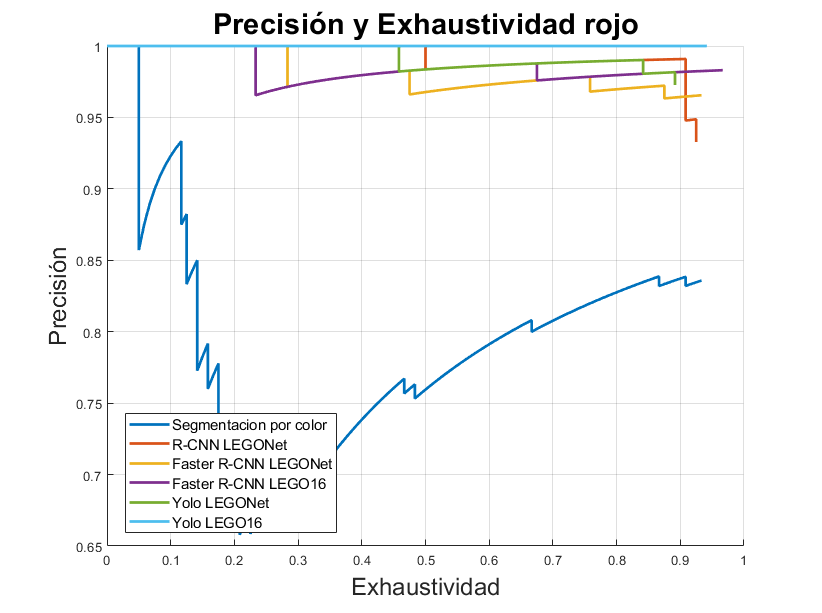
\includegraphics[width=1\textwidth]{Resultados/precision red.png}
	\end{minipage}}
  \hfill	
  \subfloat{
	\begin{minipage}[c][1\width]{0.49\textwidth}
	   \centering
	   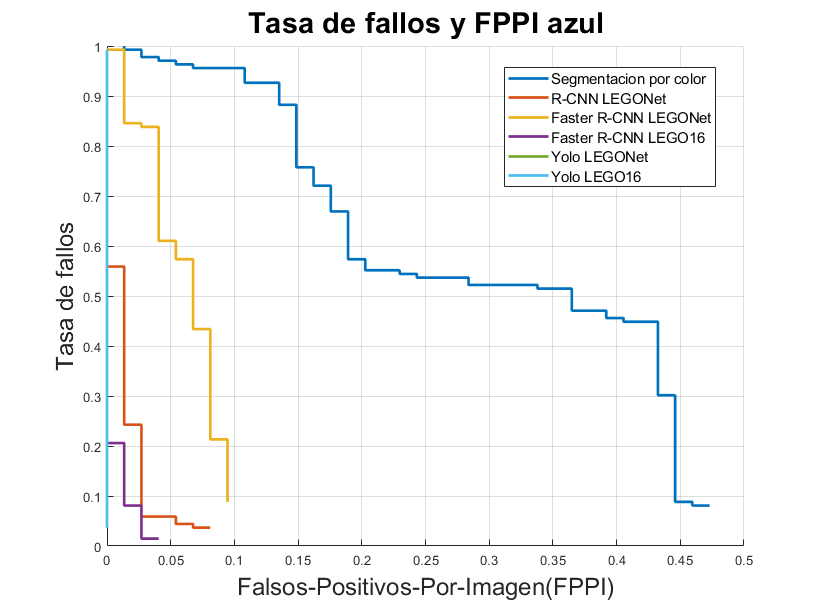
\includegraphics[width=1\textwidth]{Resultados/miss blue.png}
	\end{minipage}}
\caption{Comparativa de los métodos de segmentación al detectar piezas rojas}
\label{fig:resm2}
\end{figure}

\subsubsection*{Velocidad}
Otro factor importante de considerar a la hora de implantar un sistema es el tiempo de ejecución. Por ello durante la evaluación también se han medido los tiempos de ejecución de cada sistema. Con el fin de reflejar las diferencias en ejecución de cada sistema, las medidas han sida transformadas de décimas de segundo a imágenes por segundo. Como se puede observar, las nuevas redes neuronales no solo destacan por dar mejores resultados sino que también son más rápidas. A excepción de R-CNN cuyo rendimiento es similar al sistema clásico. Las redes que más destacan son las basadas en YOLO ya que su rendimiento es claramente superior rompiendo siempre la barrera de las 30 imágenes por segundo e incluso rompiendo la de los 60 en el caso de YOLO basado en LEGONet.

\begin{figure}[ht]  %Cajas velocidad
\vspace{-10pt}
	\centering
	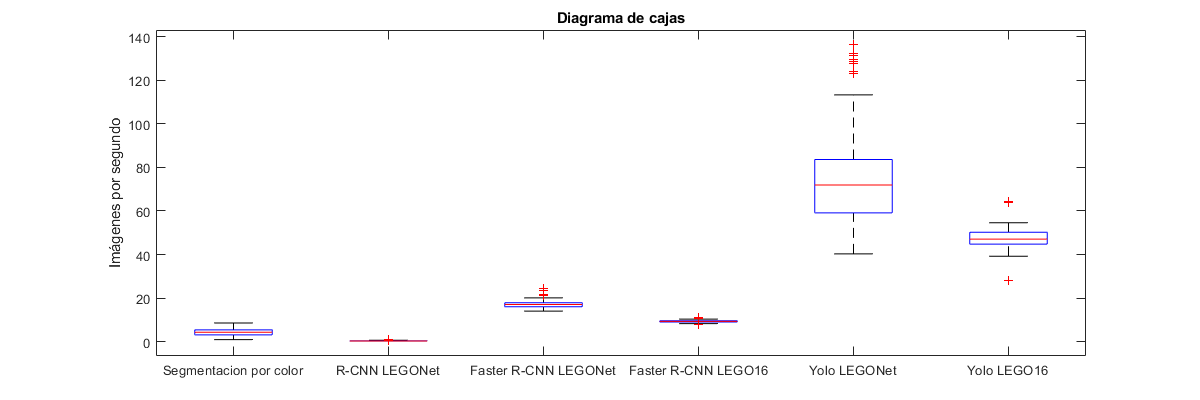
\includegraphics[width=1\textwidth]{Resultados/detectores cajas.png}
	\caption{Diagrama de cajas: Comparación de la velocidad de diferentes métodos para la segmentación (más arriba es mejor)}
	\label{fig:resm3}
\end{figure}

\subsection*{Análisis de la orientación}
También se ha llevado a cabo una evaluación de los sistemas desarrollados para el cálculo de la orientación. Es decir, el sistema clásico basado en detección de bordes y la transformada de Hough y los dos modelos de regresión basados en LEGONet y LEGO16. En el caso de estos sistemas, en la evaluación se han medido los errores medios, el error máximo, la desviación típica y la velocidad de cada sistema. De nuevo, la velocidad se ha medido en piezas de LEGO por segundo ya que refleja mejor la capacidad de cada sistema.

\begin{table}[ht] %tabla orientación precision
  \centering
    \begin{tabular}{|l|r|r|r|}
    \cline{2-4} \multicolumn{1}{r|}{} & \multicolumn{1}{l|}{Transformada de Hough} & \multicolumn{1}{l|}{LEGONet} & \multicolumn{1}{l|}{LEGO16}\\	
    \hline
    Error medio & 0.98$^{\circ}$  & 0.33$^{\circ}$ & 0.71$^{\circ}$ \\
    \hline
    Error máximo & 26$^{\circ}$  & 1.3$^{\circ}$ & 16$^{\circ}$ \\
    \hline
    Precisión & 83.67\% & 97.67\% & 79.33\% \\
    \hline
    Desviación típica & 1.82$^{\circ}$ & 0.43$^{\circ}$ & 1.23$^{\circ}$ \\
    \hline
    Piezas por segundo	&	89.7	&	74.6	&	178.5	\\
    \hline
    \end{tabular}%
  \label{tab:resm4}%
  \caption{Comparación del error medio, error máximo, precisión, desviación típica y velocidad de diferentes métodos para el cálculo de la orientación}
\end{table}

\begin{figure}[ht]  %Cajas orientación precision
	\centering
	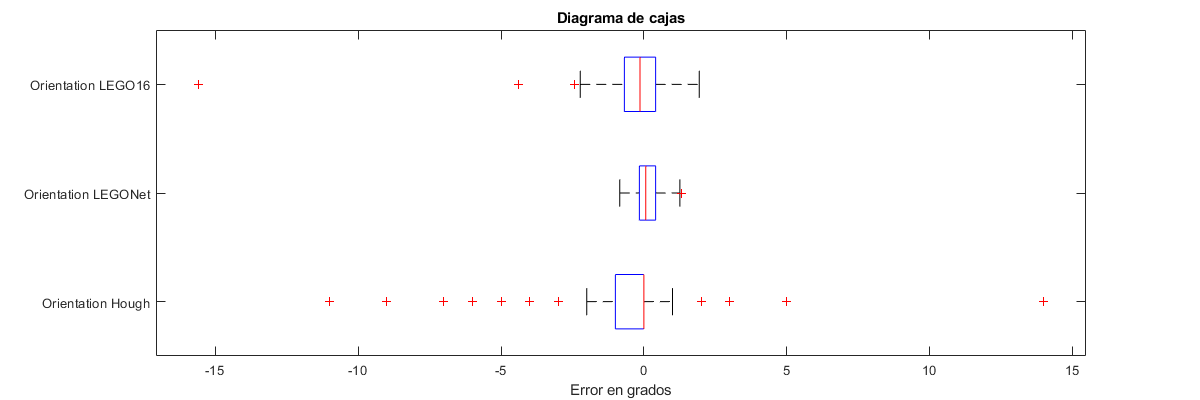
\includegraphics[width=0.95\textwidth]{Resultados/orientacion precision cajas.png}
	\caption{Diagrama de cajas: Comparación de la precisión de diferentes métodos para el cálculo de la orientación (cuanto más centrado respecto al cero y menos disperso mejor)}
	\label{fig:resm5}
\end{figure}

\section*{4. Conclusiones}
El objetivo final de este proyecto es el perfeccionamiento del sistema previamente desarrollado por Ana Berjón Valles \citep{TFGAna} mejorando la capacidad de reconocimiento. Todos los objetivos planteados durante el desarrollo del proyecto se han podido llevar a cabo y se ha mejorado en su totalidad el sistema. A continuación, se va desarrollar más en detalle los objetivos cumplidos.

Uno de los principales objetivos consiste en subsidiar los problemas del sistema antiguo ante cambios de iluminación. Como el sistema clásico se basa puramente en filtros de color y detección de borde, se ve notablemente afectado por cambios en la iluminación. Falta comprobar el funcionamiento de los sistemas desarrollados durante este proyecto en el laboratorio, pero con los resultados obtenidos durante la evaluación de estos se considera que este problema ya ha sido solventado y mitigado. Dados los resultados se recomienda para futuros proyectos la implantación del sistema basado en YOLO con LEGO16 y el modelo de regresión basado en LEGONet. También es recomendable plantearse el uso de un sistema combinado con varias redes neuronales.

Otra gran limitación del sistema anterior era los fallos debidos al análisis de profundidad. Debido al tipo de tecnología empleada para detectar la profundidad, esta se ve bastante afectada por los reflejos de las luces del laboratorio sobre las piezas de LEGO. Este problema ha podido ser solventado mediante la modificación del sistema de análisis de profundidad. Se ha introducido la posibilidad de calibrar rápidamente la cámara para poder tomar referencias de alturas. Además, se ha repartido el área de trabajo en secciones y se ha calculado la profundidad de dichas secciones con la mediana y teniendo en cuenta el entorno a la sección. De esta forma se mitiga el efecto de los reflejos.

Generalización de los algoritmos empleados. Durante el desarrollo del proyecto se ha tenido en cuenta este objetivo y es por ello que todo el procesado de la imagen no depende de la cámara, del brazo ni del laboratorio. La cámara ha sido tratada como una clase y el proceso de segmentación ya no depende tanto del calibrado de color de la cámara empleada. Además, con el procesado de la imagen de profundidad se ha creado un sistema fácil de calibrar y reutilizar para diferentes circunstancias. Esto implica que este sistema puede ser reutilizado para el reconocimiento de diferentes piezas, con diferentes cámaras y diferentes puntos de trabajo. Todo proceso que involucre al brazo robótico es llevado a cabo en forma de funciones, por ello solo modificando estas se puede implantar el sistema en cualquier otro brazo robótico del laboratorio.

Analizando el proyecto de forma global, este nuevo sistema supone un gran avance frente al anterior sistema y una vez sea implantado supondrá una gran mejora en la tecnología y capacidades de los robots industriales de Comillas ICAI.
}